\section{Transcribing}

% https://huggingface.co/learn/audio-course/en/chapter3/introduction

%1. The audio is sampled at a fixed sampling rate to amplitude values.

%2. The values are converted into spectrogram by using a Short-Time Fourier Transform, which means the wave is broken into tiny windows and Fourier transformed, so it is known how much of each specific frequency there is present. Then a spectrogram is created where the x-axis is time, the y-axis is frequency and the z-axis is the magnitude of each frequency (given by different colours)

%3. The spectrogram is converted into Mel-spectrogram, which is a scale that approximates the non-linear response humans have to sound. The linear frequencies are grouped into filters that are spread across the mel-warped frequency axis, which compresses the data so there is a high resolution at lower frequency ranges and low resolution at higher frequency ranges. (An example of how this is done could be included)

%4. The Mel-spectrogram is converted into a logarithmic scale of the magnitudes, because humans hear a sound twice as loud only if the sound is 10 times more powerful.

Before transcribing the recorded audio into text, the audio data is preprocessed into a log-mel spectrogram, which essentially simulates how humans perceive sound to differentiate words and phonemes. A log-mel spectrogram is the logarithmic representation of a mel-spectrogram. The mel scale is a perceptual scale of pitches judged by listeners to be equal in distance from one another. The Mel spectrogram is in the frequency domain, so the raw audio data is transformed from the time domain to the frequency domain using a STFT (Short-Time Fourier Transform). STFT transforms the data by splicing the the signal into overlapping windows and transforming each one seperately using a FFT (Fast Fourier Transform). Squaring the magnitude of the result gives a power spectrogram. A mel filter is then applied to the spectrogram to create a mel spectrogram. The mel filter is setup with a higher resolution at lower frequencies, where humans can discern frequencies closer to eachother and a lower resolution at higher frequencies where the human ear is less sensitive to frequency differences. The standard amount of mel channels used in the Whisper model is 80 mel channels, spaced out over the frequency spectrum. Taking the logarithm of this further approximates the values to how humans perceive sound.

The log-mel spectrogram can then be used as input for OpenAI's Whisper model for transcription. Whisper follows a transformer architecture, a deep learning model that uses attention mechanisms to focus on specific parts of the input data. Conversely to CNNs (convulutional neural networks) that process data in a sequential manner, transformers can process the entire input simultaneously, whilst performing the attention mechanisms. The usage of whisper follows the approach shown in \cref{fig:whisper_approach} 

\begin{figure}[H]
    \centering
    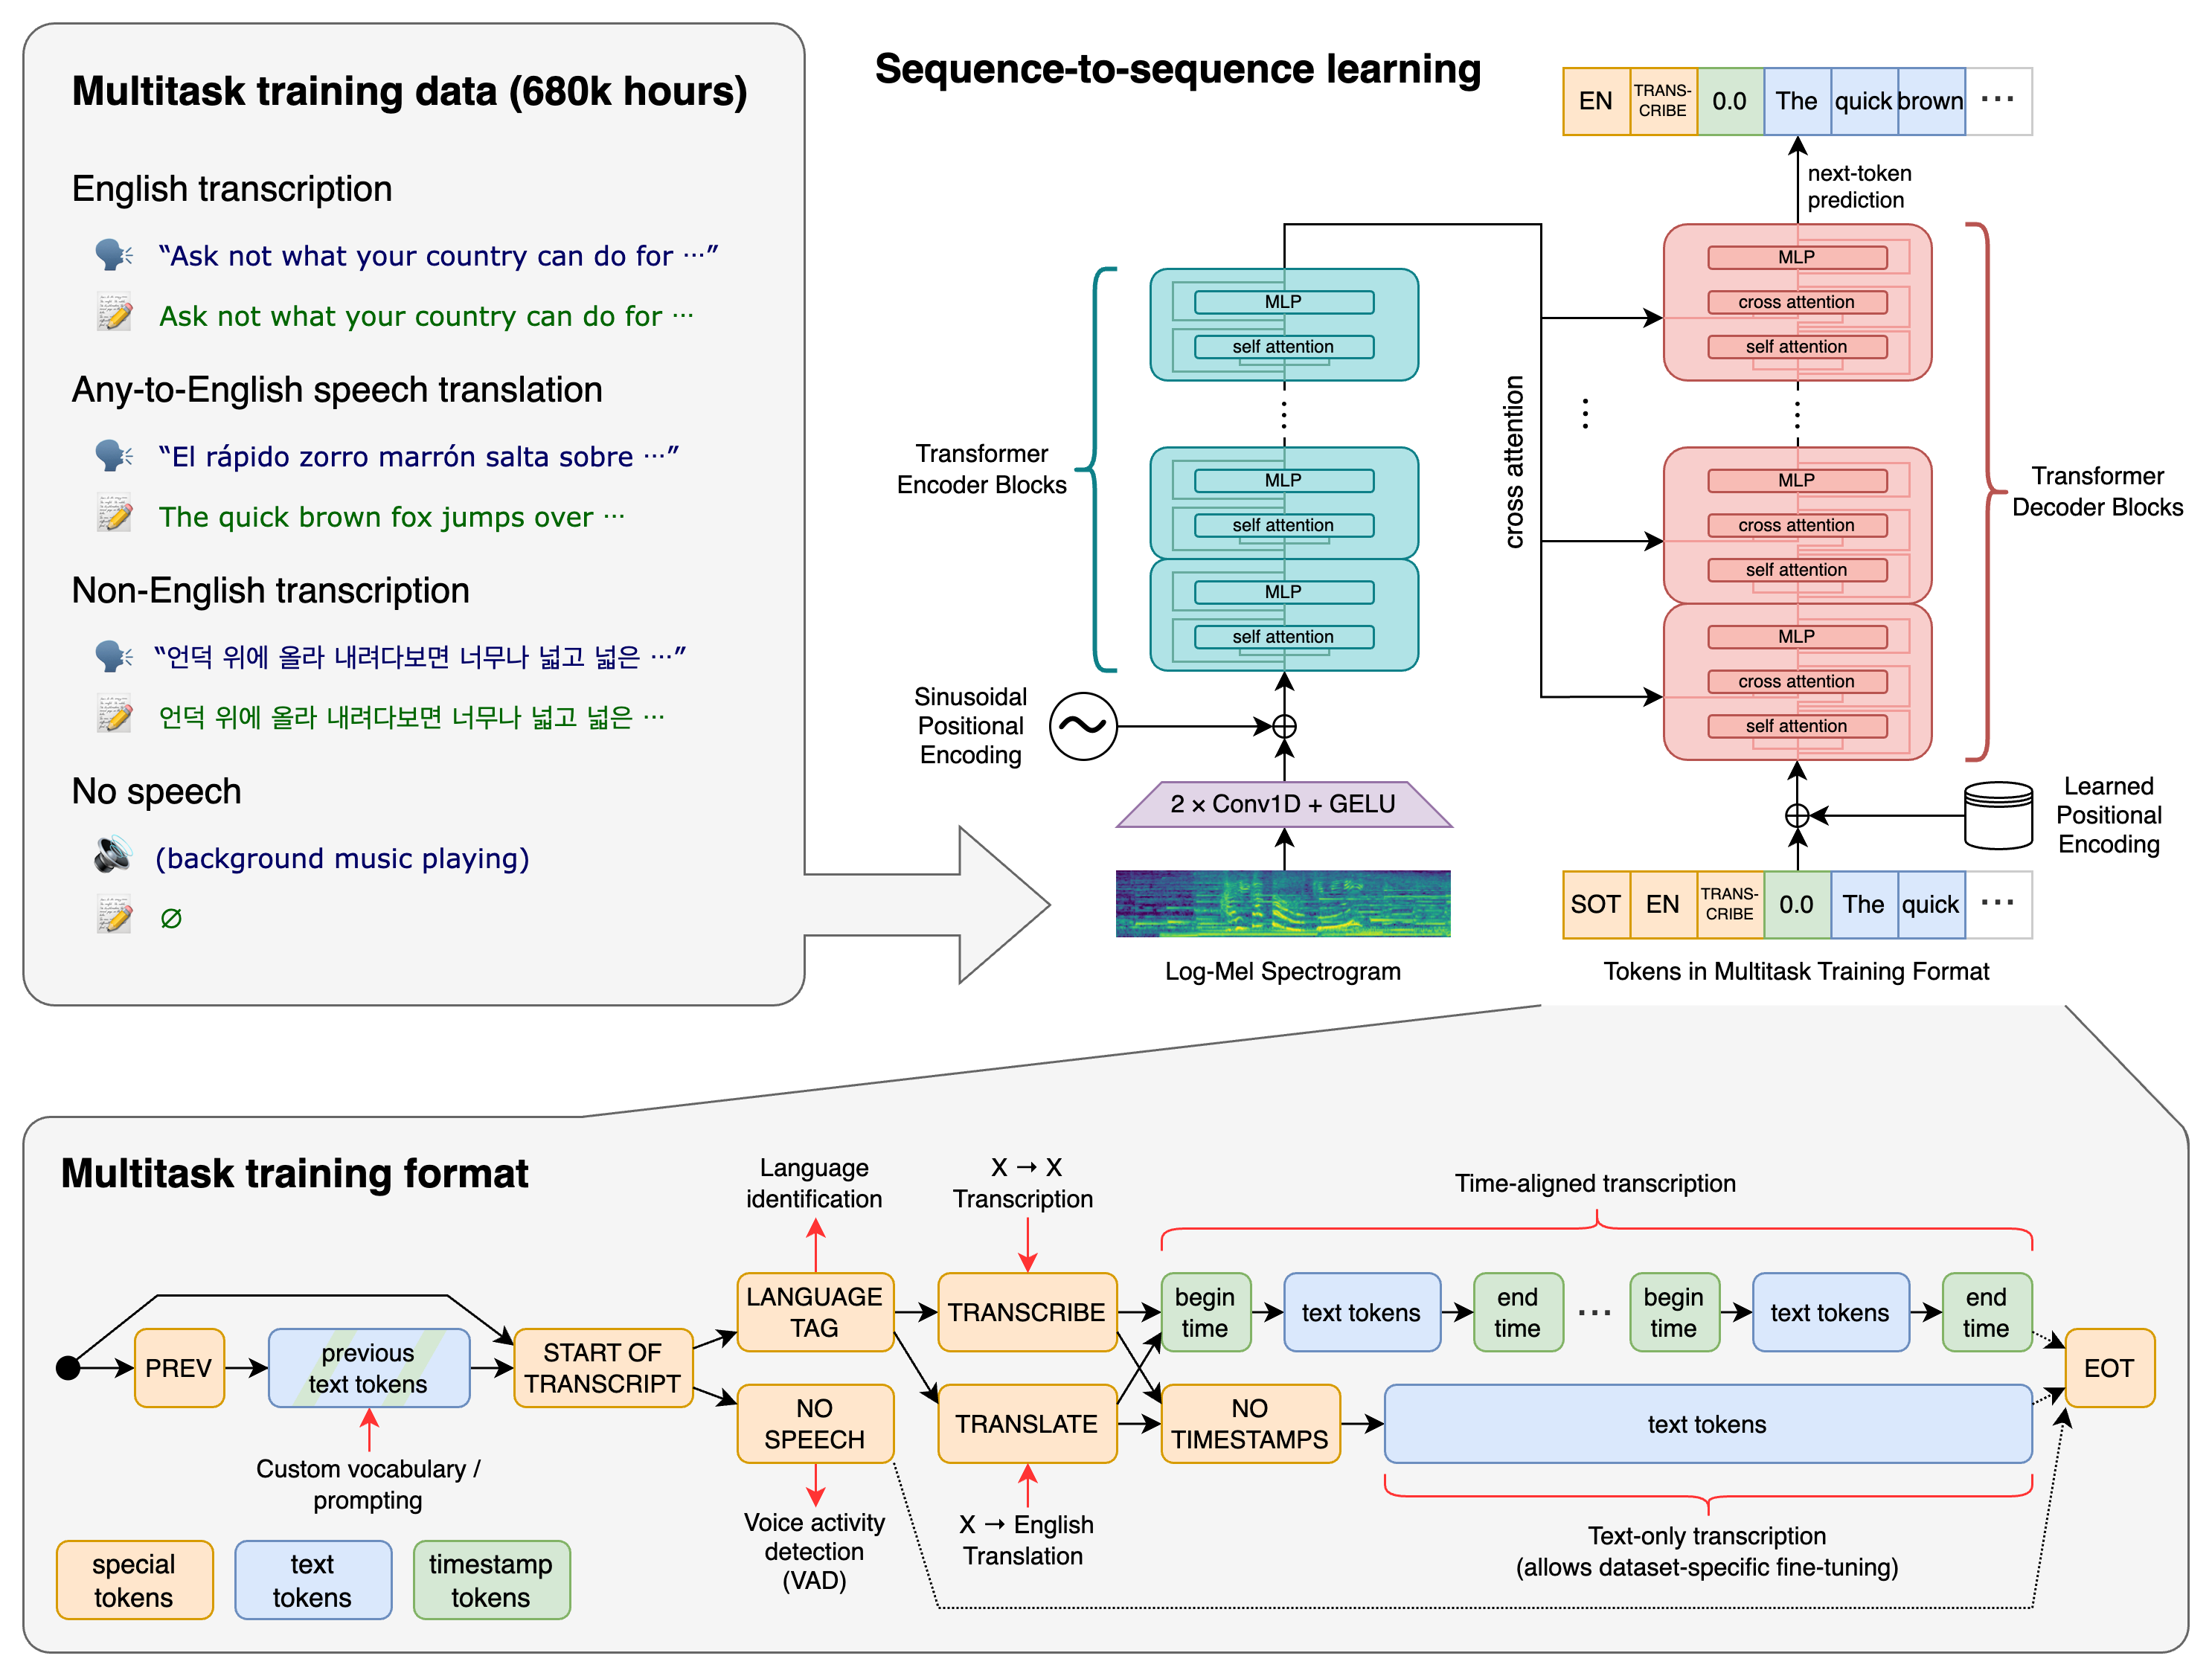
\includegraphics[width=0.7\linewidth]{Pictures/whisper_approach.png}
    \caption{Whisper approach\cite{whisper_paper}}
    \label{fig:whisper_approach}
\end{figure}

Firstly the log-mel spectrogram is processed by a CNN resulting in sequence of embeddings, which are then passed to the transformer.\cite{huggingface_whisper} The transformer then consists of a series of encoder blocks each with self attention and MLP (Multi-Layer Perceptron) layers. The output of this series is then fed into a series of decoder blocks in a process known as cross attention, where the decoder blocks besides having self attention and MLP layers also has a cross attention layer that takes the original output of the encoder series as input. After passing through the decoder series, The output can be used for token prediction. As seen on the bottom of \cref{fig:whisper_approach}, tokens will include special tokens such as language identification, timestamps and text tokens. Each token is also fed back into the decoder series to help predict the next token in the sequence. The text tokens for the entire data stream can then be converted into text using a tokenizer. This is all handled by the prebuilt Whisper model provided by OpenAI.\cite{whisper_paper}

OpenAI's whisper model has been trained on 680,000 hours of multilingual and multitask supervised data collected from the web, making it robust to background noise and accents.\cite{whisper_paper} In a noisy environment like a workshop this is especially beneficial. Whilst this project only uses the english language model, Whisper is capable of transcribing multiple languages as well as translating between them. For this project the base model is used with only the english language pack to save computational power and memory. This model has 74 million parameters. According to OpenAI's paper on the Whisper model, the base model achieves a WER (word error rate) of 4.2\% in the english language on the LibriSpeech dataset,\cite{whisper_paper} which is a standard benchmark for speech recognition models. Whisper's 4.2\% WER is one of the lowest error rates, which was another reason for choosing this exact model, and is sufficiently accurate for transcribing specific commands in a controlled environment.

Importantly OpenAI has tested the large model of whisper in a noisy environment with varying SNRs (signal-to-noise ratios). At an SNR of 0 dB the large model achieved a WER of 17\%, and at a more sensible SNR of 20 dB the WER was below 3\%.\cite{whisper_paper} Both tests running on the LibriSpeech dataset. This shows that the model is capable of functioning well even in noisy environments, and could be expected to perform well in a workshop environment. The larger model was tested on the LibriSpeech dataset with no noise, and achieved a WER of 2.7\%.\cite{whisper_paper} It can be reasonably assumed the base model will perform slightly worse in noisy environments, but still within an acceptable range for this project.

The model is used for transcription both for the purpose of identifying commands and focusing the stream for the sound localisation. The identification part is done on a seperate thread, as it is processing a larger data stream at a time, so as not to interfere with the MQTT subscriber that handles the incoming sound data.

As multiple threads need to interact with the whisper model simultaneously, a mutex lock is setup using the thread.lock\(\) function from the threading library. This ensures that only one thread can access the model at a time.

The whisper model returns a string of what has been said. As only the audio being analysed is taken into account, and commands or even words can be cut off by the boundaries of the audio stream, the audio is analysed with an overlap. In practise, this results in every audio sample being used twice with an overlap of exactly half of the analysis window. This ensures that even if a command is cut off in one sample, it will be fully present in the next sample. Since the overlap results in duplicate transcriptions, a check is needed to ensure only new information is provided for string analysis. This is done by comparing every new transcription with the previous one, and concatenating only the new part to a string that is then used for identifying commands.
